\chapter{La droite} 
\begin{eqnarray}
	f(x)=ax+b
\end{eqnarray}

exemple de la piscine, + abo
\chapter{La parabole}
\chapter{Les fonctions polynomiales}
\chapter{Les fonctions rationelles}
%\chapter{Les fonctions transcendantes}

\chapter{Algèbre élémentaire}


\begin{tikzpicture}[
    scale=5,
    axis/.style={very thick, ->, >=stealth'},
    important line/.style={thick},
    dashed line/.style={dashed, thin},
    pile/.style={thick, ->, >=stealth', shorten <=2pt, shorten
    >=2pt},
    every node/.style={color=black}
    ]
    % axis
    \draw[axis] (-0.1,0)  -- (1.1,0) node(xline)[right]
        {$G\uparrow/T\downarrow$};
    \draw[axis] (0,-0.1) -- (0,1.1) node(yline)[above] {$E$};
    % Lines
    \draw[important line] (.15,.15) coordinate (A) -- (.85,.85)
        coordinate (B) node[right, text width=5em] {$Y^O$};
    \draw[important line] (.15,.85) coordinate (C) -- (.85,.15)
        coordinate (D) node[right, text width=5em] {$\mathit{NX}=x$};
    % Intersection of lines
    \fill[red] (intersection cs:
       first line={(A) -- (B)},
       second line={(C) -- (D)}) coordinate (E) circle (.4pt)
       node[above,] {$A$};
    % The E point is placed more or less randomly
    \fill[red]  (E) +(-.075cm,-.2cm) coordinate (out) circle (.4pt)
        node[below left] {$B$};
    % Line connecting out and ext balances
    \draw [pile] (out) -- (intersection of A--B and out--[shift={(0:1pt)}]out)
        coordinate (extbal);
    \fill[red] (extbal) circle (.4pt) node[above] {$C$};
    % line connecting  out and int balances
    \draw [pile] (out) -- (intersection of C--D and out--[shift={(0:1pt)}]out)
        coordinate (intbal);
    \fill[red] (intbal) circle (.4pt) node[above] {$D$};
    % line between out og all balanced out :)
    \draw[pile] (out) -- (E);
\end{tikzpicture}

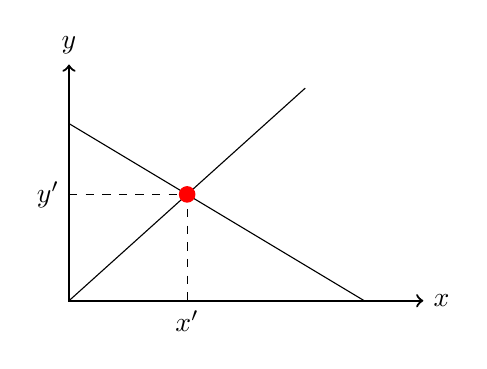
\begin{tikzpicture}[scale=1.5]
    % Draw axes
    \draw [<->,thick] (0,2) node (yaxis) [above] {$y$}
        |- (3,0) node (xaxis) [right] {$x$};
    % Draw two intersecting lines
    \draw (0,0) coordinate (a_1) -- (2,1.8) coordinate (a_2);
    \draw (0,1.5) coordinate (b_1) -- (2.5,0) coordinate (b_2);
    % Calculate the intersection of the lines a_1 -- a_2 and b_1 -- b_2
    % and store the coordinate in c.
    \coordinate (c) at (intersection of a_1--a_2 and b_1--b_2);
    % Draw lines indicating intersection with y and x axis. Here we use
    % the perpendicular coordinate system
    \draw[dashed] (yaxis |- c) node[left] {$y'$}
        -| (xaxis -| c) node[below] {$x'$};
    % Draw a dot to indicate intersection point
    \fill[red] (c) circle (2pt);
\end{tikzpicture}
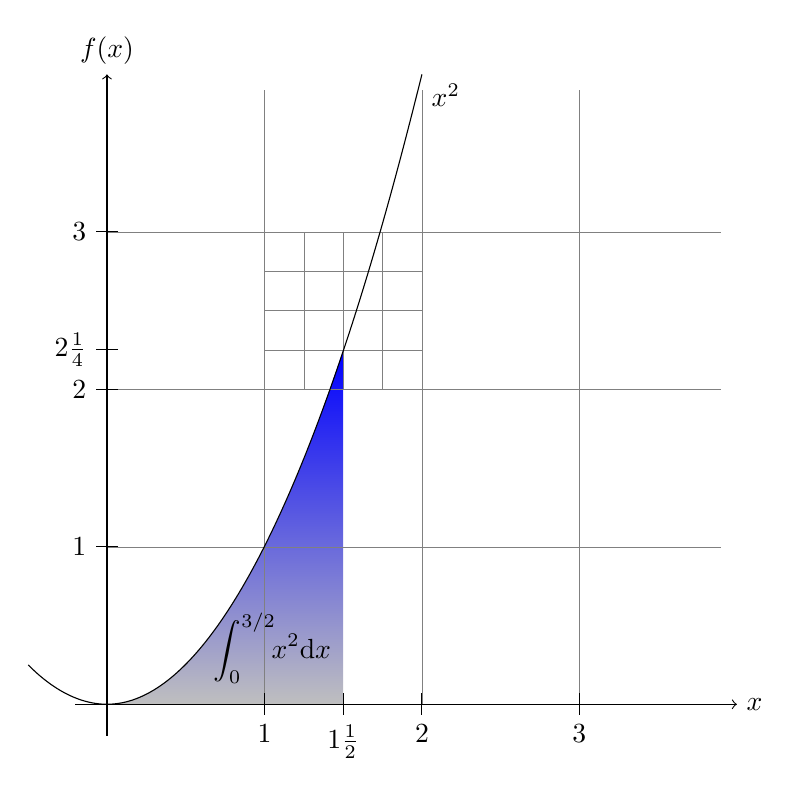
\begin{tikzpicture}[scale=2]
  \shade[top color=blue,bottom color=gray!50] 
      (0,0) parabola (1.5,2.25) |- (0,0);
  \draw (1.05cm,2pt) node[above] 
      {$\displaystyle\int_0^{3/2} \!\!x^2\mathrm{d}x$};

  \draw[style=help lines] (0,0) grid (3.9,3.9)
       [step=0.25cm]      (1,2) grid +(1,1);

  \draw[->] (-0.2,0) -- (4,0) node[right] {$x$};
  \draw[->] (0,-0.2) -- (0,4) node[above] {$f(x)$};

  \foreach \x/\xtext in {1/1, 1.5/1\frac{1}{2}, 2/2, 3/3}
    \draw[shift={(\x,0)}] (0pt,2pt) -- (0pt,-2pt) node[below] {$\xtext$};

  \foreach \y/\ytext in {1/1, 2/2, 2.25/2\frac{1}{4}, 3/3}
    \draw[shift={(0,\y)}] (2pt,0pt) -- (-2pt,0pt) node[left] {$\ytext$};

  \draw (-.5,.25) parabola bend (0,0) (2,4) node[below right] {$x^2$};
\end{tikzpicture}

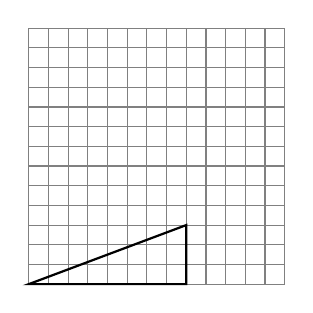
\begin{tikzpicture}[scale=0.25] 
\draw [gray] (0,0) grid (13,13); 
\draw [thick] 
(0,0) -- ++(8,0) -- ++(0,3) -- cycle; 
\end{tikzpicture}

\begin{comment}
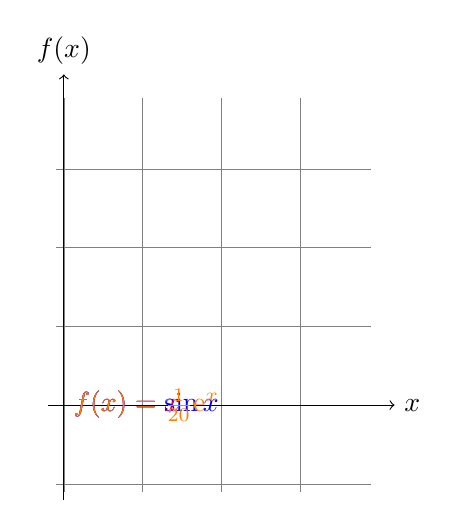
\begin{tikzpicture}[domain=0:4]
    \draw[very thin,color=gray] (-0.1,-1.1) grid (3.9,3.9);
    \draw[->] (-0.2,0) -- (4.2,0) node[right] {$x$};
    \draw[->] (0,-1.2) -- (0,4.2) node[above] {$f(x)$};
    \draw[color=red] plot[id=x] function{x} 
        node[right] {$f(x) =x$};
    \draw[color=blue] plot[id=sin] function{cos(x)} 
        node[right] {$f(x) = \sin x$};
    \draw[color=orange] plot[id=exp] function{0.05*exp(x)} 
        node[right] {$f(x) = \frac{1}{20} \mathrm e^x$};
\end{tikzpicture}
\end{comment}